\documentclass[12pt]{article}
\usepackage{xcolor}
\usepackage{lipsum}
\usepackage{amssymb,amsmath}
\usepackage{graphicx}
\usepackage{geometry}
\usepackage[hang]{footmisc}
\usepackage{enumitem}
\setlist[enumerate]{topsep=.2em, itemsep=.2em}
\usepackage[colorlinks,linkcolor=violet,anchorcolor=blue,citecolor=blue]{hyperref}
\geometry{left=3.28cm,right=3.28cm,top=3cm,bottom=3.5cm}
\linespread{1.2}
\setlength{\parskip}{0.4\baselineskip}
\title{}
\author{}
\date{}
% define counters for comment and subcomment
\newcounter{comment}
\setcounter{comment}{1}
\newcounter{subcomment}[comment]
\setcounter{subcomment}{0}

\makeatletter
\renewcommand{\fnum@figure}{Fig.~R\thefigure}
\makeatother
\renewcommand*{\thefootnote}{R\arabic{footnote}}

\renewcommand{\thecomment}{Comment\,\arabic{comment}} 
\renewcommand{\thesubcomment}{\thecomment.\arabic{subcomment}} 
% comment
\newcommand{\comment}[1]{\stepcounter{comment} \bigskip \noindent 
	\textsl{{\fontseries{b}\selectfont \thecomment\,:}\medskip\\ #1}\smallskip\par}
% subcomment
\newcommand{\subcomment}[1]{\stepcounter{subcomment} \bigskip \noindent 
	\textsl{{\fontseries{b}\selectfont \thesubcomment\,:}\medskip\\ #1}\smallskip\par}
% reply
\newcommand{\reply}[1]{\noindent \textbf{\fontseries{b}\selectfont Response\,:}\medskip\\#1\medskip\par}
% added content
\newcommand{\add}[1]{\noindent\textcolor{blue}{#1}}
\newcommand{\pos}[1]{\noindent\emph{\small#1}}
\newcommand{\D}{\mathrm{d}}
\setlength{\footnotesep}{14pt}
\setlength{\skip\footins}{24pt}
\begin{document}

	{\centering
	\textsc{{\LARGE Response Letter of Applied Optics\\ \medskip manuscript 264478}}\par}\vspace{2em}

	{\small \noindent
	{\fontseries{b}\selectfont Manuscript title}: Camera response prediction for various capture settings using the spectral sensitivity and crosstalk model\smallskip\\
	\noindent
	{\fontseries{b}\selectfont Authors}: XX\smallskip\\
	\noindent
	{\fontseries{b}\selectfont Corresponding Author}: XX (xxx@zju.edu.cn)
	\vspace{2em}
	
	\noindent
	Dear Prof.\ XX,\bigskip
	
	\noindent
	Thank you for giving us an opportunity for revising our manuscript. Your comments and those of the reviewer were highly insightful and enabled us to greatly improve the quality and understanding of our manuscript. This article has been carefully revised according to these comments, and the details are explained in the following ``\textit{Response to Reviewer's Comments}'' section, in which the words in \add{blue} color represent the modified contents in the revised version. For more details, a ``\textit{List of Changes in the Revised Manuscript}'' and a ``\textit{Response to Pre-Production Review}'' are provided as well.
	
	\noindent
	In addition, we submitted a file named \verb|AO264478_RedLined.pdf| to the online system, in which the removed contents of the revised version are crossed out with a single line and colored \textcolor{red}{red}, whereas the added contents are underlined with a squiggle and colored \textcolor{blue}{blue}. Besides, the line numbers, which would be used in ``\textit{Response to Reviewer's Comments}'' and ``\textit{List of Changes in the Revised Manuscript}'' section, are marked on the outer margin of pages for a more direct localization.
	
	\noindent
	We hope that, after the revision, our manuscript would be acceptable for Applied Optics.
	
	\noindent
	Thank you very much for your attention.\medskip
	
	\noindent
	Sincerely,\vfill
	
	\noindent
	Author\\[.1em]
	College of Optical Science and Engineering\\
	Zhejiang University\\
	Hangzhou 310027, China\\
	Email: xxx@zju.edu.cn}
		
	\clearpage
	
	\section*{\fontseries{b}\selectfont Response to Reviewer's Comments}\medskip
		
	\noindent\underline{\fontseries{b}\selectfont{\large Reviewer \texttt{\#}1}}\medskip
	
	\subcomment{
		Introduction, paragraph 3, the last sentence: please add reference.}
	
	\reply{
		Thanks for the comment. We have already added the reference:
		
		\pos{In Section Reference, page 9, line 115--117}\\
		\add{[3] A.~Getman, T.~Uvarov, Y.~Han, B.~Kim, J.~Ahn, and Y.~Lee, ``Crosstalk, color tint and shading correction for small pixel size image sensor,'' in ``International Image Sensor Workshop,'' (2007), pp.\ 166–-169}.
		
		Reference~3 is cited to support the viewpoint, which is mentioned in the last sentence of paragraph 3 in Introduction, that the crosstalk effect among adjacent pixels is ignorable in high-accuracy color reproduction. Besides reference~3, we also provide supplementary material to support this conclusion by comparing our model with those without considering the crosstalk effect. The details will be discussed in the \hyperlink{comment5}{response to comment~5.}}
	
	\subcomment{
		Introduction, paragraph 5, the last sentence: In other words \ldots: camera responses are determined by SPD, reflectance and spectral sensitivity function of filters. If the spectral sensitivity functions are not important, why do you need estimate the sensitivity function? Otherwise, you can use the empirical method converting RGB to CIELAB or CIEXYZ.}
	
	\hypertarget{comment1.2}{}
	\reply{
		Since the statement of ``the camera spectral sensitivity are not concerned'' may be misleading to reviewers and readers, we modify this sentence to:
		
		\pos{In Section~1: Introduction, page 2, line 2--6}\\
		\add{Considering that the camera spectral sensitivity is only a bridge that links the physical properties of real world, e.g., surfaces’ spectral radiances, to the digital output responses, the core of this study would be the prediction of the camera responses rather than the spectral sensitivity}.
		
		When said ``it is the camera responses, rather than the spectral sensitivity itself, that are concerned'', we did not intend to indicate that the camera spectral sensitivity functions are not important, but just to point out it is only an intermediary in our model, not the final goal.
		
		The original intention of proposed camera response formation model is to construct a bridge linking the radiometric properties of objects, for example, the spectral radiance of surfaces, to camera's final digital responses. In the whole model, although camera's spectral sensitivity function undoubtedly plays an indispensable role, without which the conversion from physical properties to digital quantities is impossible to be accomplished, it is not our major focus---our focus is to use it, as well as crosstalk matrix and the nonlinear parameters, to predict the output digital responses as accurately as possible.
		
		In our study, we convert the camera RGB to CIELAB or CIEXYZ only for evaluating how \textit{perceptually accurate} could we achieve, but not for investigating camera characterization itself. If one wish the predicted responses were \textit{numerically} close to the actual responses, there is no need to perform colorimetric characterization, we can simply set the relative errors in RGB space as the cost function---this is actually how the preceding studies did.}\label{1.2}
	
	\subcomment{
		Eq.(1): authors did not consider the noise.}
	
	\hypertarget{comment1.3}{}
	\reply{
		A very scrupulous comment! We have added the noise to Eq.~(1) and explained why the noise is trivial in our model:
		
		\pos{In Section~2.A: Response formation model, page 3, line 5--7}\\
		\add{\begin{equation}
			p(\mathbf{x}) = f_\text{S}\cdot\Big(\int_\tau Q(\mathbf{x})\,\D{t}+c_1\Big)+n\,,
			\end{equation}
		\ldots where $n$ is the random noise with zero mean and finite variance, thus can be neglected by applying an average filter.}}

		The actual camera responses in our study were extracted from images of the color checker by applying spatial average filters to the central regions of every color patches. The size of spatial average filters is $22\times22$, in other words, the actual response of one color sample is the mean value of 484 pixels, so we believe that the noise is negligible after the filtering.
		
	\subcomment{
		The paragraph before Eq.(1): the conversion of the camera responses obtained with ISO800 and 1/125 s to those obtained with ISO800 and 120 s is valid only when the camera responses are linear (no saturation). The range of normalized camera responses under different conditions is from 0.9 to 1.1. This may be due to the noise especially at high ISO level signal to noise ratio is low.}
	
	\reply{
		We have added a figure (Fig.~3, in revised version) to prove that the responses of D3x has a good linearity with respect to exposure time, so this conversion is valid. We also add some information following the original sentence:
		
		\pos{In Section~2.A: Response formation model, page 2, line 85--87}\\
		\add{This conversion is valid only when the camera responses are linear with respect to exposure time, which can be demonstrated by Fig. 3}.
		
		In fact, Fig.~2 is only a qualitative illustration. The positive slope in Fig.~2 is enough to support our point that the exposure time and ISO sensitivity are nonequivalent in the response formation model, otherwise these polylines should be near-horizontal.
		
		We think that the range of normalized camera responses under different conditions is from 0.9 to 1.1, may not be resulted from the noise, which is negligible as explained in the \hyperlink{comment1.3}{response to comment~1.3}, but is mainly due to the nonequivalence of exposure time and ISO sensitivity. Please allow us to describe how Fig.~2 was obtained.
		
		Let's take the blue patch in color checker for example. After we had obtained the camera responses of blue patch under five different capture settings (ISO\,100+1/15s, ISO\,200+1/30s, ISO\,400+1/60s, ISO\,800+1/120s and ISO\,1600+1/240s), we divided these five responses simultaneously by the response under setting ISO100+1/15s. Same operations were applied to other patches, that is why the normalized responses under setting ISO100+1/15s for all patches are equal to one. If this normalization were not performed, it would be difficult to depict this trend for all patches, because the responses of different patches cover a huge range of intensity.
		
		According to the nonequivalence of exposure time and ISO sensitivity in Eq.(1), the ideal range of normalized camera responses under different conditions should be greater than 1. The normalized responses of several patches under ISO\,200+1/30s, however, are below 1, this may be due to the inevitable measuring errors or other instability of the system. Though there may be some exceptional patches, the overall trend of Fig.~2 is quite evident.}
	
	\subcomment{
		The paragraph after following Eq.(1): $Q(x)$ is\ldots please add ``this is also called quantum efficiency''. Please use $t$ as the integration time, since $T$ is also used as transmittance of the filter.}
	
	\reply{
		Thanks again for meticulosity. We have corrected the notation of the integration time and replaced $T$ with $\tau$, since the symbol $t$ is the variable of integration.
		
		As for the comment about the quantum efficiency's notation, we beg to differ. In Eq.(1), $Q$ is not the quantum efficiency, but is the amount of electrons converted from photons by the sensor at a pixel. In Eq.(2) of revised manuscript, $Q(x)$ is defined as:
		\begin{equation*}
		Q(\mathbf{x}) = \int_\Omega{}E(\lambda,\mathbf{x})S_\text{Q}(\lambda)\,\D{\lambda}\,,
		\end{equation*}
		where $S_\text{Q}(\lambda)$ is the quantum efficiency of the sensor, according to our definition.
		
		The statement we made about the quantum efficiency were more ambiguous than intended, so we have adjusted to the text to be clearer. We have exchanged the order of Eq.(2) and Eq.(3) in the original manuscript: first give a definition of the relationship of $Q(\mathbf{x})$ with $S_\text{Q}(\lambda)$ and $E(\lambda,\mathbf{x})$ (spectral irradiance), then introduce the ``physical term'':
		\begin{equation*}
		\Phi(\mathbf{x}) = \int_\tau Q(\mathbf{x})\,\D{t}\,,
		\end{equation*}
		and finally take the nonlinear parameters into consideration:
		\begin{equation*}
		p(\mathbf{x}) = f_\text{S}\cdot\bigg[\Big(\int_\tau Q(\mathbf{x})\,\D{t}+c_1\Big)^\beta+c_2\bigg]\,.
		\end{equation*}}
	
	\subcomment{
		Eq.(2): I suggest that authors investigate the linearity of the camera. The power ($\beta$) is needed for the region near saturation.}
	
	\reply{
		We conducted a supplementary experiment to investigate the linearity of D3x. The camera responses with respect to exposure time are plotted in Fig.~3 of revised version.
		
		In the supplementary experiment, we captured five neutral patches of X-Rite ColorChecker Classic (\texttt{\#}19--23) under the different exposure time from 1/160s to 1/1.3s, with the interval of 1/3Ev, thus obtained totally 22 kinds of exposure time. The experimental operations are very similar to those detailed in section 3.A, paragraph 2--4.
		
		In order to get enough number of samples in the scatter diagram, we normalized the responses of five patches as follows (takes green channel for example):
		
		For color patch \texttt{\#}20, its spectral radiance measured by Konica Minolta CS-2000 spectroradiometer is about 0.656 times as large as the spectral radiance of patch \texttt{\#}19 in visible range, so we multiplied the real exposure time of patch \texttt{\#}20 by 0.656 and plotted these ``shifted'' points. The responses shift is illustrated in Fig.~R\ref{fig:ResponsesShift}.
		
		\begin{figure}[tbp]
			\centering
			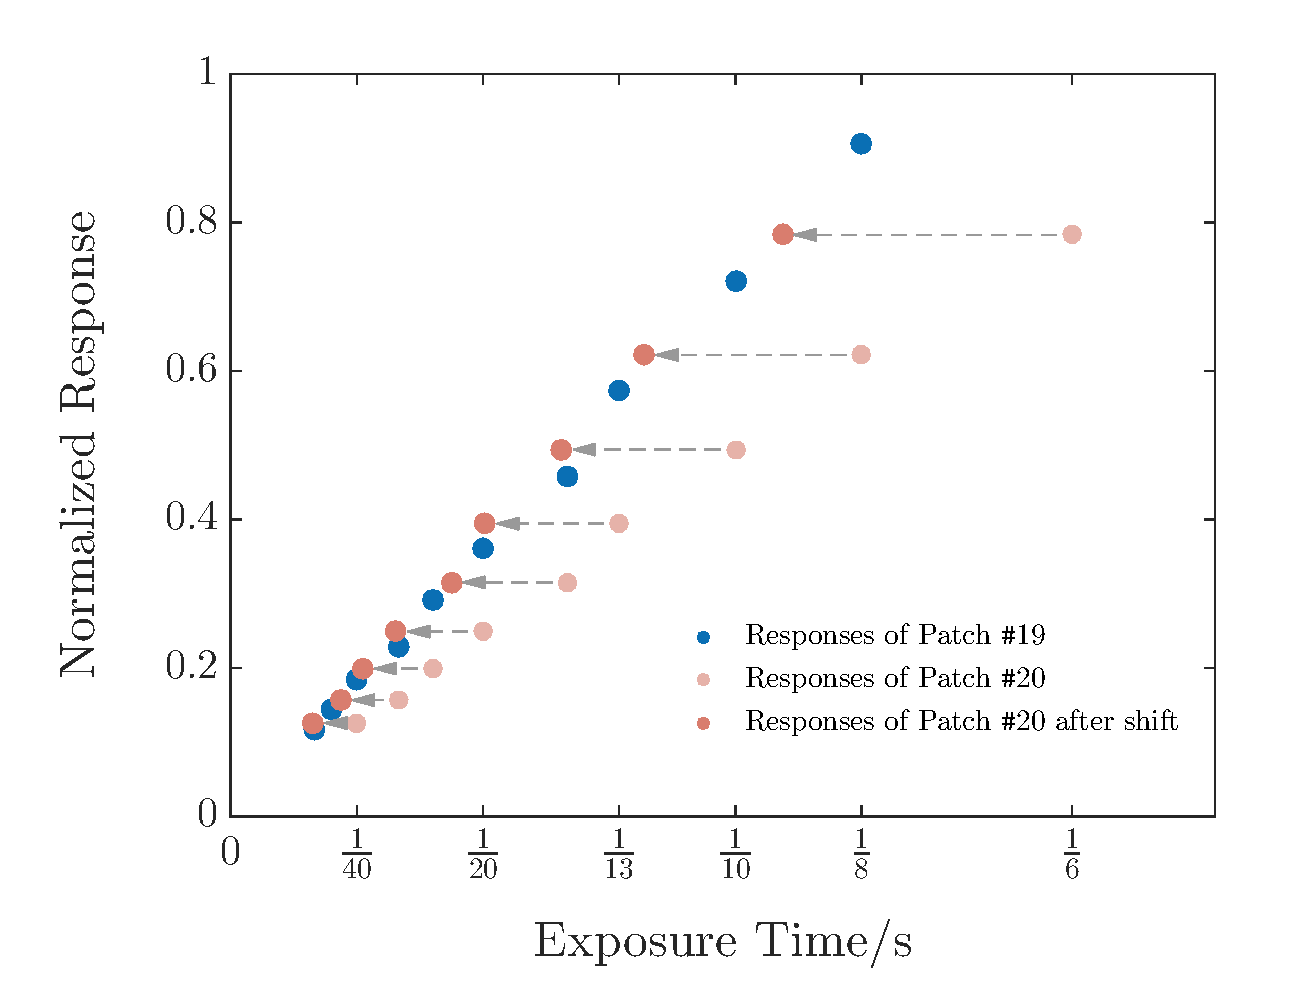
\includegraphics[width=.65\linewidth]{ResponsesShift.eps}
			\caption{The responses shift from patch \texttt{\#}20 to patch \texttt{\#}19.}
			\label{fig:ResponsesShift}
		\end{figure}
		
		The same operations were done for patches \texttt{\#}21, \texttt{\#}22 and \texttt{\#}23. That's how Fig.~3 of revised version is obtained.
		
		We consider this normalization to be valid based on (a) The spectral reflectances of neutral patches are of a very strong similarity in shape, only differing in their amplitudes, thus they can be approximately modulated only by a scalar; (b) According to the definition of the physical term $\Phi(\mathbf{x})$ in our model:
		\begin{equation*}
		\Phi(\mathbf{x}) = \tau Q(\mathbf{x}) = \int_\Omega\tau E(\lambda,\mathbf{x})S_\text{Q}(\lambda)\,\D{\lambda} = \int_\Omega\tau R(\lambda,\mathbf{x})L(\lambda)S_\text{Q}(\lambda)\,\D{\lambda}\,,
		\end{equation*}
		the exposure time $\tau$ and the spectral reflectance of target $R(\lambda,\mathbf{x})$ are commutative, so we can multiply the scalar of reflectance to the exposure time; (c) The dark current of D3x is close to zero, as we discussed in section~4.A of original manuscript, thus we can neglect the offset when applying shift; and (d) The investigation of the linearity is only a qualitative analysis, we did not use it for any numerical calculation.
		
		We calculated the Standardized Residual Sum of Squares (STRESS) of scatters in Fig.~3 of revised version, and got the result of 3.58\%. STRESS is essentially a measure of fit for evaluating the agreement between two variables [\footnotetext[1]{\hypertarget{ref1}{P.~Garc\'{\i}a, R.~Huertas, M.~Melgosa, and G.~Cui, ``Measurement of the relationship between perceived and computed color differences,'' J.\ Opt.\ Soc.\ Am.\ A \textbf{24}, 1823--1829 (2007)}}\hyperlink{ref1}{R1}]. Here we use it as an index to evaluate the linearity between the exposure time and the normalized responses. The STRESS value is always falling into the range of 0--100, in such a way that higher STRESS values mean poorer agreement between the two data sets. The STRESS should equal zero for a perfect agreement, and a STRESS value of 3.58 indicates a disagreement of about 3.58\%. The STRESS of scatters in Fig.~3 is calculated as follows:
		\begin{equation*}
		\textit{STRESS} = \bigg(\,\frac{\sum(\tau-fp)^2}{\sum f^2p^2}\,\bigg)^{\frac{1}{2}}\times 100\%\,,
		\end{equation*}
		where $p$ is the normalized response and
		\begin{equation*}
		f = \frac{\sum\tau^2}{\sum\tau p}\,.
		\end{equation*}

		From Fig.~3 of revised version and the STRESS index, it is considered that the linearity of camera responses with respect to exposure time is very good, even in the region near saturation, being consistent with the power of the nonlinear parameters after optimization ($\beta=0.9875$).}
	
	\subcomment{
		Section B Training samples selection: why training samples which are linearly independent are more noise-resistant?}
	
	\reply{
		Nice point. It is our negligence for missing the explanation about their causality. Let's arrange the spectral radiances of training samples into a matrix $\mathbf{A}$, each row of which corresponds to one sample. For one group of training samples that are more linearly independent than any others, the condition number of the corresponding $\mathbf{A}$ is the smallest. In the field of numerical analysis, a large condition number implies that the problem is ill-posed, in other words, the matrix $\mathbf{A}$ might be close to being singular, although it is not. Once the problem is ill-posed, even a small error (noise) in the data gets amplified by the large inverse of $\mathbf{A}$, producing a large deviation in the solution.
		
		We have modified the statement in the original manuscript to make it clearer:
		
		\pos{In Section 3.B, page 8, line 3--4}\\
		\add{\ldots to keep away from being ill-posed.}
		
		We have also added a reference to support this point:
		
		\pos{In Section Reference, page 11, line 35--37}\\
		\add{[21] P.~C.~Hansen and D.~P.~O'Leary, ``The use of the l-curve in the regularization of discrete ill-posed problems,'' SIAM Journal on Scientific Computing \textbf{14}, 1487–-1503 (1993).},\\
		in which the author pointed out, ``In all but trivial deconvolution problems, the continuous problem is ill-posed in the sense that small changes in the data can cause arbitrarily large changes in the solution,\ldots''.}
	
	\comment{
		When convert RGB to CIELAB, 66 coefficients ($3\times22$) need to be estimated, but the number of training samples is 48, which is less than the number of coefficients. Does the number of training samples is good or not?}
	
	\hypertarget{comment2}{}
	\reply{
		There might be some misunderstanding about the purpose of colorimetric characterization. As we explained in the \hyperlink{comment1.2}{response to comment~1.2}, the colorimetric characterization, i.e., the calculation of $3\times22$ conversion matrix $\mathbf{M}$, is not one of step in constructing camera responses formation model, although it is applied to the predicted responses $\hat{\boldsymbol{\rho}}$ (expanded form of $\hat{\mathbf{p}}$) during every iteration. 
		
		The conversion matrix $\mathbf{M}$ was calculated, or say, the colorimetric characterization was accomplished, using the responses of 96, rather than 48, color samples captured under the setting of 1/15s exposure time and ISO\,100 (discussed in the second paragraph after Eq.(11)). We apply $\mathbf{M}$ to both the actually recorded responses $\mathbf{p}$ and the predicted responses $\hat{\mathbf{p}}$, only in order to evaluate how perceptually close they are.}
	
	\comment{
		When you calculate CIELAB, do you use actual SPD of the light box or not?}
	
	\reply{
		Yes. We used Konica Minolta CS-2000 spectroradiometer to measure the spectral radiance of each color patch, and then integrated them with CIE1931 color matching functions to get the actual XYZ tristimulus values. Finally, we converted CIEXYZ to CIELAB using forward transformation formula.}
	
	\comment{
		I suggest that the authors compare the performance of their method with other empirical methods for digital camera characterization, e.g.: use the same polynomial regression method to convert obtained RGB to CIELAB.}
	
	\reply{
		The suggested comparison is interesting and would provide additional information about camera characterization, however it may fall outside the scope of this study. As we explained in the \hyperlink{comment1.2}{response to comment~1.2} and the \hyperlink{comment2}{response to comment~2}, the camera colorimetric characterization is a tool that allow us to evaluate the closeness of our predicted responses to the actual ones in a perceptually uniform color space, but dose not provide more information or influence the performance to our model.
		
		In addition, since our model is proposed to predict the camera responses under different capture settings, it is crucial that the color correction method should be invariant with respect to the change of illumination
		intensity. Other empirical methods, e.g., polynomial regression, cannot guarantee the invariance of chromaticities when the camera exposure and/or scene irradiance changes, so it could be expected that the empirical methods would deteriorate the color prediction accuracy.}
	
	\comment{
		I suggest that the authors compare their estimated spectral sensitivity function with those obtained from other methods (PCA based, pseudo inverse based).}
	
	\hypertarget{comment5}{}
	\reply{
		This is a helpful suggestion. We have added the comparison to both section~4.A Parameters estimation and section~4.B Response prediction.
		
		In section~4.A, we compare our estimated spectral sensitivity function with those obtained by pseudo inverse based, radial basis function based and PCA based methods. The pseudo inverse based method is similar to that used to obtain the initial parameters of our model, but only with regularization constraint. The radial basis function based method, which is claimed to be the best one in various basis function based methods [\footnotetext[2]{\hypertarget{ref2}{H.~Zhao, R.~Kawakami, R.~T.~Tan, and K.~Ikeuchi, ``Estimating basis functions for spectral sensitivity of digital cameras,'' in ``Meeting on Image Recognition and Understanding,'' (2009), 1.}}\hyperlink{ref2}{R2}], approximates the camera spectral sensitivity of each channel by a linear combination of a small number of radial basis functions:
		\begin{equation*}
		S^{(k)}(\lambda) = \sum_{i=0}^{D}a^{(k)}_i\exp\bigg(-\frac{(\lambda-\mu_i)^2}{\sigma^2}\bigg)\,.
		\end{equation*}
		
		Since the author of [\hyperlink{ref2}{R2}] did not give appropriate values for $\mu_i$ and $\sigma$, we use the camera spectral sensitivities database as training set to find the optimized ones. The spectral sensitivities database we used are from project [\footnotetext[3]{\hypertarget{ref3}{J.~Jiang, D.~Liu, J.~Gu, and S.~S\"{u}sstrunk, ``What is the space of spectral sensitivity functions for digital color cameras?'' in ``Workshop on Applications of Computer Vision (WACV) 2013 IEEE,'' (2013), pp.\ 168-–179.}}\hyperlink{ref3}{R3}] and [\footnotetext[4]{\hypertarget{ref4}{R.~Kawakami, Z.~Hongxun, R.~T.~Tan, and K.~Ikeuchi, ``Camera spectral sensitivity and white balance estimation from sky images,'' International Journal of Computer Vision (2013).}}\hyperlink{ref4}{R4}]. We also add a reference for the latter:
		
		\pos{In Section Reference, page 11, line 44--46}\\
		\add{[24] R.~Kawakami, Z.~Hongxun, R.~T.~Tan, and K.~Ikeuchi, ``Camera spectral sensitivity and white balance estimation from sky images,'' International Journal of Computer Vision (2013)}.
		
		PCA was performed on all 40 cameras and all Nikon cameras to investigate the difference across different types of cameras, as suggested in [\hyperlink{ref3}{R3}], therefore we obtain two sets of results, notated with ``PCA-All'' and ``PCA-Nikon'' respectively. The principal components are obtained from two sets of training database, and the scores of each principal component for D3x are found so that the predicted spectral sensitivity causes the minimum color prediction error. Same as [\hyperlink{ref3}{R3}], we use the first two principal components.
		
		The comparison of the estimated spectral sensitivities obtained by different methods are plotted in Fig.~11 of revised version. All functions are normalized so as to have the same peak value, since the other methods can only estimate the relative spectral sensitivity for each channel independently.
		
		We added some contents to explain these comparisons in the revised manuscript:
		
		\pos{In Section~4.A: Parameters estimation, page 9, line 15--28}\\
		\add{We also compared our estimated camera spectral sensitivity with those obtained by other prevalling methods. Fig.~11 plots five sets of spectral sensitivities estimated by pseudo inverse~[6], radial basis functions network(RBFN)~[8], principal component analysis (PCA)~[9], and our proposed method. The camera spectral sensitivities database to be implemented by PCA and RBFN were downloaded from \url{http://www.cis.rit.edu/~dxl5849/projects/camspec/} and \url{http://www.cvl.iis.u-tokyo.ac.jp/~rei/research/cs/index.html}~[24], respectively. The notation ``PCA-All'' in Fig.~11 corresponds to the result obtained by performing PCA to all 40 cameras, and ``PCA-Nikon'' to only 12 Nikon cameras. The pseudo inverse method used here is similar to that described in section~B.2 but only with the regularization constraint.}
		
		In section~4.B, we compared the color prediction performance of our estimated spectral sensitivity function with others. Fig.~10(a), Fig.~11(a) and Fig.~12(a) of original version are substituted by three new figures, in which the CIEDE2000 color differences $\Delta{}E_{00}$ under different capture settings, for the five methods, are plotted for comparison. These figures clearly show that our model has a significant superiority of color prediction over others. The traditional methods, without considering the nonequivalence between the exposure time and ISO, goes down when the capture settings are different from the one under which they were calculated.
		
		We have also added some contents to explain these comparisons in the revised manuscript:
		
		\pos{In Section~4.B: Response prediction, page 9, line 34--45}\\
		\add{Since the spectral sensitivities estimated by other methods are relative data, they are normalized so that the peak value of each channel is equal to our result, as demonstrated in Fig.~11. Thanks to the introduction of crosstalk matrix and the nonlinear parameters, our model show a significant superiority of color prediction over others, especially when the capture setting varies. The prediction accuracy of the traditional methods, without considering the nonequivalence between the exposure time and ISO, goes down when the capture settings are different from the one under which they were calculated, yet the proposed model keeps at the same level.}}

	\bigskip
	
	The more detailed list of all the changes in this paper is given in the following ``\textit{List of changes in the revised manuscript}'' section.
	
	Special thanks for your kind and helpful comments.
	
	\clearpage
	
	\section*{\fontseries{b}\selectfont List of changes in the revised manuscript}
	
	Please note that, the line marks in the following correspond to the positions of the \textit{\underline{differentiated version}} (\verb|AO264478_RevisedDiff.pdf|), rather than the revised or original version.
	
	\bigskip
	
	\noindent\underline{\textbf{{\large In Section~1: Introduction}}}
	
	\begin{enumerate}
		\item Page 1, line 30, reference\,3 was added.
		
		\item Page 1, line 35, the word ``specified'' was removed.
		
		\item Page 2, line 1, the phrase ``color reproduction'' was changed to ``color rendering''.
		
		\item Page 2, line 2--6, the misleading statement about the role of camera spectral sensitivity in our model was modified to be clearer.
	\end{enumerate}
	
	\noindent\underline{\textbf{{\large In Section~2.A: Response formation model}}}
	
	\begin{enumerate}[resume]
		\item Page 2, line 35, the phrase ``the captured image'' was changed to ``image''.
		
		\item Page 2, line 43--45, the sentence structures were modified.
		
		\item Page 2, line 46--50, the statement about camera responses, which may lead to misunderstanding, was removed.
		
		\item Page 2, line 55, the phrase ``RGB triplet'' was changed to ``triplet''.
		
		\item Page 2, line 65, the word ``keeping'' was changed to ``with''.
		
		\item Page 2, line 69, the phrase ``averaging filter'' was changed to ``average filter''. Same modification was also applied to Page~3, line~9.
		
		\item Page 2, line 85--87, we added some supplementary description to Fig.~2.
		
		\item Page 2, line 88, the word ``inequivalence'' was changed to ``nonequivalence''. Same modifications were also applied to Page~3, line~11 and Page~9, line 43.
		
		\item Page 3, line 3, the missed symbol ``$\mathbf{x}$'' was added. Same modification was also applied to Page~3, line~58.
		
		\item Page 3, Eq.~(1), the notation of the integration time was changed to ``$\tau$''. Same modifications were also applied to Page~3, line~3, 11, 23, 30, Eq.~(3) and Page~4, Eqs.~(6), (7), (8), (10).
		
		\item Page 3, Eq.~(1), the noise term was added, and some explanation about noise was added in Page~3, line~5--7.
		
		\item Page 3, line 14--22, the introduction of the relationship among the amount of electrons, the quantum efficiency and the spectral irradiance was brought forward. The original one in Page~3, line~43--51 was removed.
		
		\item Page 3, line 28--30, the introduction of the physical term $\phi(\mathbf{x})$ was moved here. The original one in Page~3, line~41--43 was removed.
		
		\item Page 3, top of the right column, a figure investigating the linearity of camera was added (Fig.~3).
		
		\item Page 3, line 38, the equation mark number ``(2)'' was changed to ``(3)''.
		
		\item Page 3, line 51--56, the explanation of Fig.~3 was added.
		
		\item Page 3, line 57, the phrase ``the spectral power distribution (SPD) of irradiance'' was changed to ``the spectral irradiance''.
		
		\item Page 3, line 59, the phrase ``the SPD of scene's radiance'' was changed to ``the scene's spectral rradiance''.
		
		\item Page 4, Eq.~(7) (bottom of the left column), the crosstalk coefficients $c$ was changed to $C$.
	\end{enumerate}
	
	\noindent\underline{\textbf{{\large In Section~2.B: Spectral sensitivity and parameters estimation}}}
	
	\begin{enumerate}[resume]
		\item Page 5, line 12, the figure mark number ``4'' was changed to ``5''. Similar modifications were also applied to Page~6, line~40, Page~7, line 61, 66, 92, Page~8, line~20, 21, 26, 33, 41 and Page~9, line~27, 48, 58, 77, 82.
		
		\item Page 5, line 65, the scalar ``$s$'' was changed to ``$c$''.
	\end{enumerate}
	
	\noindent\underline{\textbf{{\large In Section~3.B: Training samples selection}}}
	
	\begin{enumerate}[resume]
		\item Page 7, line 100, the word ``including'' was changed to a colon.
		
		\item Page 8, line 3--4, we added some contents to make the statement of noise-resistant clearer.
		
		\item Page 8, line 4, reference\,21 was added.
		
		\item Page 8, line 5, the word ``few'' was changed to ``small''.
		
		\item Page 8, line 9, the phrase ``$\ell2$-norm'' was changed to ``$\ell_2$-norm''.
	\end{enumerate}
	
	\noindent\underline{\textbf{{\large In Section~4.A: Parameters estimation}}}
	
	\begin{enumerate}[resume]
		\item Page 9, line 15--28, we added the comparison of estimated camera spectral sensitivities obtained by different methods. and add the explanation about Fig.~11. Reference\,24 was also added.
		
		\item Page 10, top, a new figure was added in which the estimated spectral sensitivities obtained by different methods were compared.
	\end{enumerate}
	
	\noindent\underline{\textbf{{\large In Section~4.B: Response prediction}}}
	
	\begin{enumerate}[resume]
		\item Page 9, line 30--31, the word ``under'' was changed to ``for'', and we added a phrase ``obtained by five methods''.
		
		\item Page 9, line 34--45, the new analysis about Fig.~12(a) was added. The explanation about the error bar was brought forward, the original one in Page~9, line~50--51 was removed.
		
		\item Page 9, line 46, the sentence was completed with ``It should be noted that since the\ldots''.
		
		\item Page 9, line 49, the word ``even'' was added.
		
		\item Page 9, line 55--56, the phrase ``color difference $\Delta{}E_{00}$ averaging over\ldots'' was changed to ``color difference $\Delta{}E_{00}$ of our model averaged over\ldots''.
		
		\item Page 9, line 58--59, the word ``investigated'' was changed to ``compare'', and the phrase ``our response formation model'' was changed to ``our model with the others''.
		
		\item Page 9, line 64, we added a phrase ``our model of''.
		
		\item Page 10, left column below the table, we replaced the original bar chart with a new chart (Fig.~12(a)), in which the color prediction accuracy among different methods were compared. Similar modifications were also applied to Fig.~13(a) and Fig.~14(a).
		
		\item Page 9, line 70, we added a word ``again''.
		
		\item Page 9, line 87, we added a phrase ``of our model''.
		
		\item Page 9, line 88, we added a phrase ``by our model''.
		
		\item Page 9, line 91, we changed the preposition ``in'' to ``of''.
	\end{enumerate}
	
	\noindent\underline{\textbf{{\large In Section: Acknowledgments}}}
	
	\begin{enumerate}[resume]
		\item Page 9, line 111--113, we added acknowledgments section to manuscript.
	\end{enumerate}
	
	\noindent\underline{\textbf{{\large In Section: Reference}}}
	
	Three new references were added.
	\begin{enumerate}[resume]
		\item Page 10, line 1--3, ``[3] A.~Getman, T.~Uvarov, Y.~Han, B.~Kim, J.~Ahn, and Y.~Lee, `Crosstalk, color tint and shading correction for small pixel size image sensor,' in `International Image Sensor Workshop,' (2007), pp. 166–169.''
		
		\item Page 11, line 35--37, ``[21] P.~C.~Hansen and D.~P.~O'Leary, `The use of the l-curve in the regularization of discrete ill-posed problems,' SIAM Journal on Scientific Computing \textbf{14}, 1487–1503 (1993).''
		
		\item Page 11, line 44--46, ``[24] R.~Kawakami, Z.~Hongxun, R.~T.~Tan, and K.~Ikeuchi, `Camera spectral sensitivity and white balance estimation from sky images,' International Journal of Computer Vision (2013).''
	\end{enumerate}
	
	\bigskip\medskip
	
	Correspondingly, the sequence numbers of the figures and references have also been reordered according to the corresponding citation positions of the paper.
	
	Many thanks for your time.
	
	\clearpage
	
	\section*{\fontseries{b}\selectfont Response to Pre-Production Review}
	
	\setcounter{comment}{0}
	
	\comment{
		Please upload electronic figure files in TIFF, EPS, or JPEG format.}
	
	\reply{
		We have uploaded EPS figure files to online system.}
	
	\comment{
		For free color figures online-only please submit electronic art files following instructions given at the journal website: \url{https://www.osapublishing.org/submit/style/coloronline.cfm}.  Use these instructions to submit figures that are or grayscale only: \url{https://www.osapublishing.org/ao/submit/style/default.cfm}.}
	
	\reply{
		We have submitted the electronic art files of Fig.~1 to Fig.~14.
		
		Fig.~3 and Fig.~11 are newly added in the revised manuscript; Fig.~12(a), Fig.~13(a) and Fig.~13(a) are substitutes for Fig.~10(a), Fig.~11(a) and Fig.~12(a) of the original version, respectively.}
	
	\comment{
		Please ensure that all references, figures and tables are called out in the text. Please also check the ordering of your reference, figure and table call outs. If they are out of order it could cause delays with publishing your article.}
	
	\reply{
		We have checked them after revision.}
	
	\comment{
		When citing a reference you must include publication, title, authors, and page numbers. You may not use "et al" to indicate additional authors.}
	
	\reply{
		We have carefully checked the references to make sure that they contain the necessary information.}
	
	\comment{
		After revision, please make sure that the references are cited in numerical order; renumber references if necessary. Please remove any duplicate references and renumber accordingly.}
	
	\reply{
		We have checked and renumber them carefully.}
	
	\comment{
		We estimate that your manuscript will be approximately 10 journal pages.  We will proceed with the understanding, according to your response on the Prism website, that you have agreed to pay overlength page charges at the rate of \$300 per page if the final article exceeds ten pages.  The exact page count will be determined after typesetting.}
	
	\reply{
		Yes, we agree to pay the overlength page charges if the final article exceeds ten pages. However, we hope to keep the length of this paper within 10 pages as far as possible.}
	
	
	
\end{document}